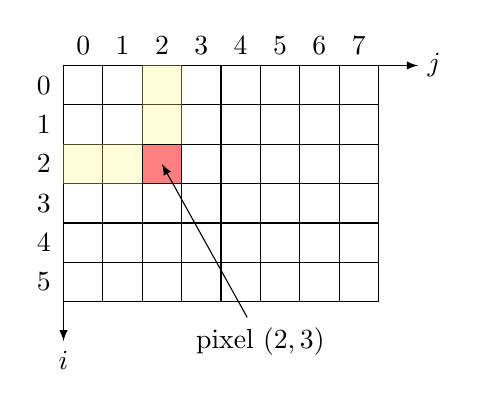
\begin{tikzpicture}[scale=0.5]
	\foreach \i in {0,1,...,6}
	{
		\draw (0,\i) -- ++(8,0);
	}
	\foreach \i in {0,1,...,5}
	{
		\node at (-0.5, 5.5 - \i) {$\i$};
	}	
	\foreach \j in {0,1,...,8}
	{
		\draw (\j,0) -- ++(0,6);
	}
	\foreach \j in {0,1,...,7}
	{
		\node at (\j + 0.5, 6.5) {$\j$};
	}		
	\draw[-latex] (0,6) -- ++(0,-7) node[anchor=north] {$i$};		
	\draw[-latex] (0,6) -- ++(9,0) node[anchor=west] {$j$};

    \pause
    \draw [draw=none, fill=yellow!50, opacity=0.3] (0,3) rectangle (3,4);
    \draw [draw=none, fill=yellow!50, opacity=0.3] (2,3) rectangle (3,6);
    \draw[fill=red!50] (2,3) rectangle ++(1,1);
    \node (a) at  (5,-1) {pixel $(2,3)$};
    \draw[-latex] (a) -- (2.5,3.5);
	
\end{tikzpicture} 